\documentclass[12pt,utf8,notheorems,compress]{beamer}
\usepackage{etex}

\usepackage[ngerman]{babel}

\usepackage{ragged2e}
\usepackage{multicol}
\usepackage{tabto}

\usepackage[protrusion=true,expansion=true]{microtype}

\setlength\parskip{\medskipamount}
\setlength\parindent{0pt}

\title{Zahlen, die größer als unendlich sind}
\author[Tag der Mathematik 2016]{Ingo Blechschmidt}
\date{5. März 2016}

\usetheme{Warsaw}
\usecolortheme{seahorse}
%\usefonttheme{default}?
%\usepackage{kurier}?
\usefonttheme{serif}
%\usepackage{libertine}?
%\usepackage{mathpazo}
\usepackage[T1]{fontenc}
\usepackage{libertine}
\useinnertheme{rectangles}

\setbeamertemplate{title page}[default][colsep=-1bp,rounded=false,shadow=false,bg=white]
\setbeamertemplate{frametitle}[default][colsep=-2bp,rounded=false,shadow=false,center]

\setbeamertemplate{headline}{}
\setbeamertemplate{navigation symbols}{}

\newcommand*\oldmacro{}%
\let\oldmacro\insertshorttitle%
\renewcommand*\insertshorttitle{%
  \oldmacro\hfill\insertframenumber\,/\,\inserttotalframenumber\hfill}

\newcommand{\hil}[1]{{\usebeamercolor[fg]{item}{\textbf{#1}}}}

\newcommand{\imgslide}[2]{
  \begin{frame}\frametitle{#1}
    \centering
    \includegraphics[height=0.85\textheight]{#2}
    \par
  \end{frame}
}

\newcommand{\imgslideslogan}[3]{
  \begin{frame}\frametitle{#1}
    \centering
    \includegraphics[height=0.75\textheight]{#2}
    \par
    #3
    \par
  \end{frame}
}

\begin{document}

\imgslide{Wundersame Formen}{mandelbrot}

\begin{frame}\frametitle{Unendlichkeit}
  \begin{columns}[c]
    \begin{column}{0.5\textwidth}
      \centering

      % http://vladimir-bulatov.deviantart.com/art/Circle-Limit-I-285568627 (Escher)
      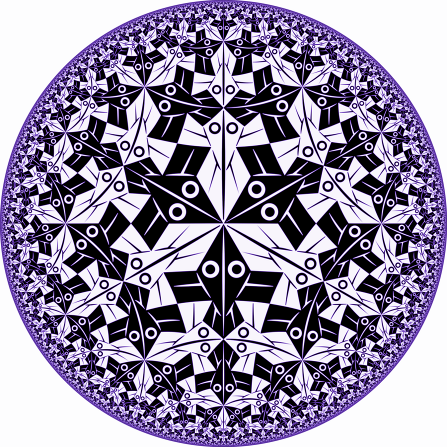
\includegraphics[width=0.6\textwidth]{infinity-circle}
      \bigskip

      % https://society6.com/product/infinity-symbol-stars-galaxy-space_print
      
\includegraphics[width=0.6\textwidth]{infinity-space}
    \end{column}
    \begin{column}{0.5\textwidth}
      % http://www.tfo-meran.it/wp-content/uploads/2011/03/fraktal49-Kopie.jpg
      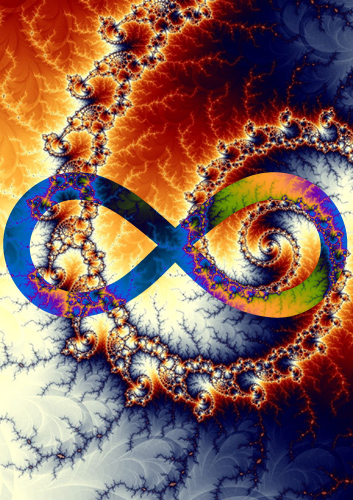
\includegraphics[height=0.8\textheight]{infinity-fractal}
    \end{column}
  \end{columns}
\end{frame}

% im Hintergrund abspielen:
% 10_Hours_of_Infinite_Fractal_and_Falling_Shepard_s_Tone
% https://www.youtube.com/watch?v=u9VMfdG873E

\imgslide{Unendlichkeit}{infinity-mirrors}
% xawtv -c /dev/video0  # jemand aus dem Publikum kann nach vorne kommen

\imgslideslogan{Ordinalzahlen}{infinite-queue}{\hil{Ordinalzahlen messen Anordnung.}}

\begin{frame}\frametitle{Hilbert und Noether}
  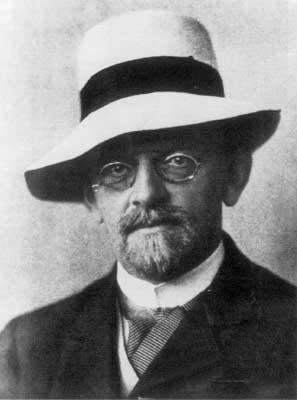
\includegraphics[width=0.45\textwidth]{hilbert}
  \hfill
  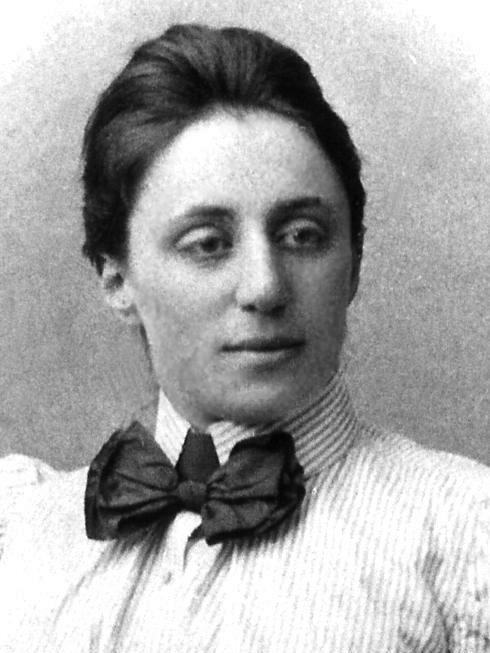
\includegraphics[width=0.45\textwidth]{noether}
\end{frame}

\imgslideslogan{Kardinalzahlen}{hilberts-hotel}{\hil{Kardinalzahlen messen Anzahl.}}
% Gewittergeräusche

\begin{frame}\frametitle{Aleph}
  \centering
  \Huge\hil{\scalebox{7}{$\aleph$}}
  \par
\end{frame}

\begin{frame}
  \centering
  \hil{In der Mathematik gibt es eine unendliche Hierarchie \\ immer größer
  werdender Unendlichkeiten.}
  \medskip

  {\quad\,\,\,}
\includegraphics[width=3cm]{gregor}
  \medskip

  Lust auf spannende Mathematik abseits des Schulunterrichts? \\
  In kleinen Gruppen auf dem Campus? Oder lieber per Post?

  Dann komm zum \hil{Matheschülerzirkel Augsburg}!
  \par
\end{frame}

\end{document}

% für sshlatex

\includegraphics{mandelbrot}
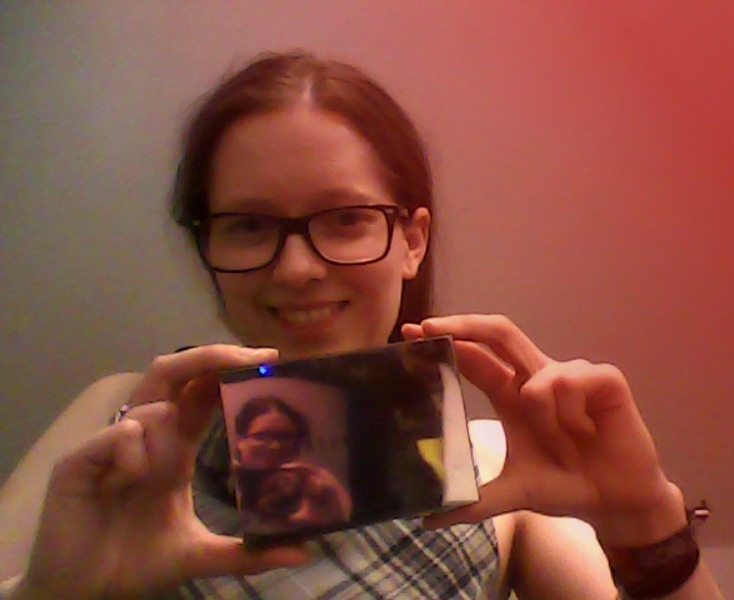
\includegraphics{infinity-mirrors}
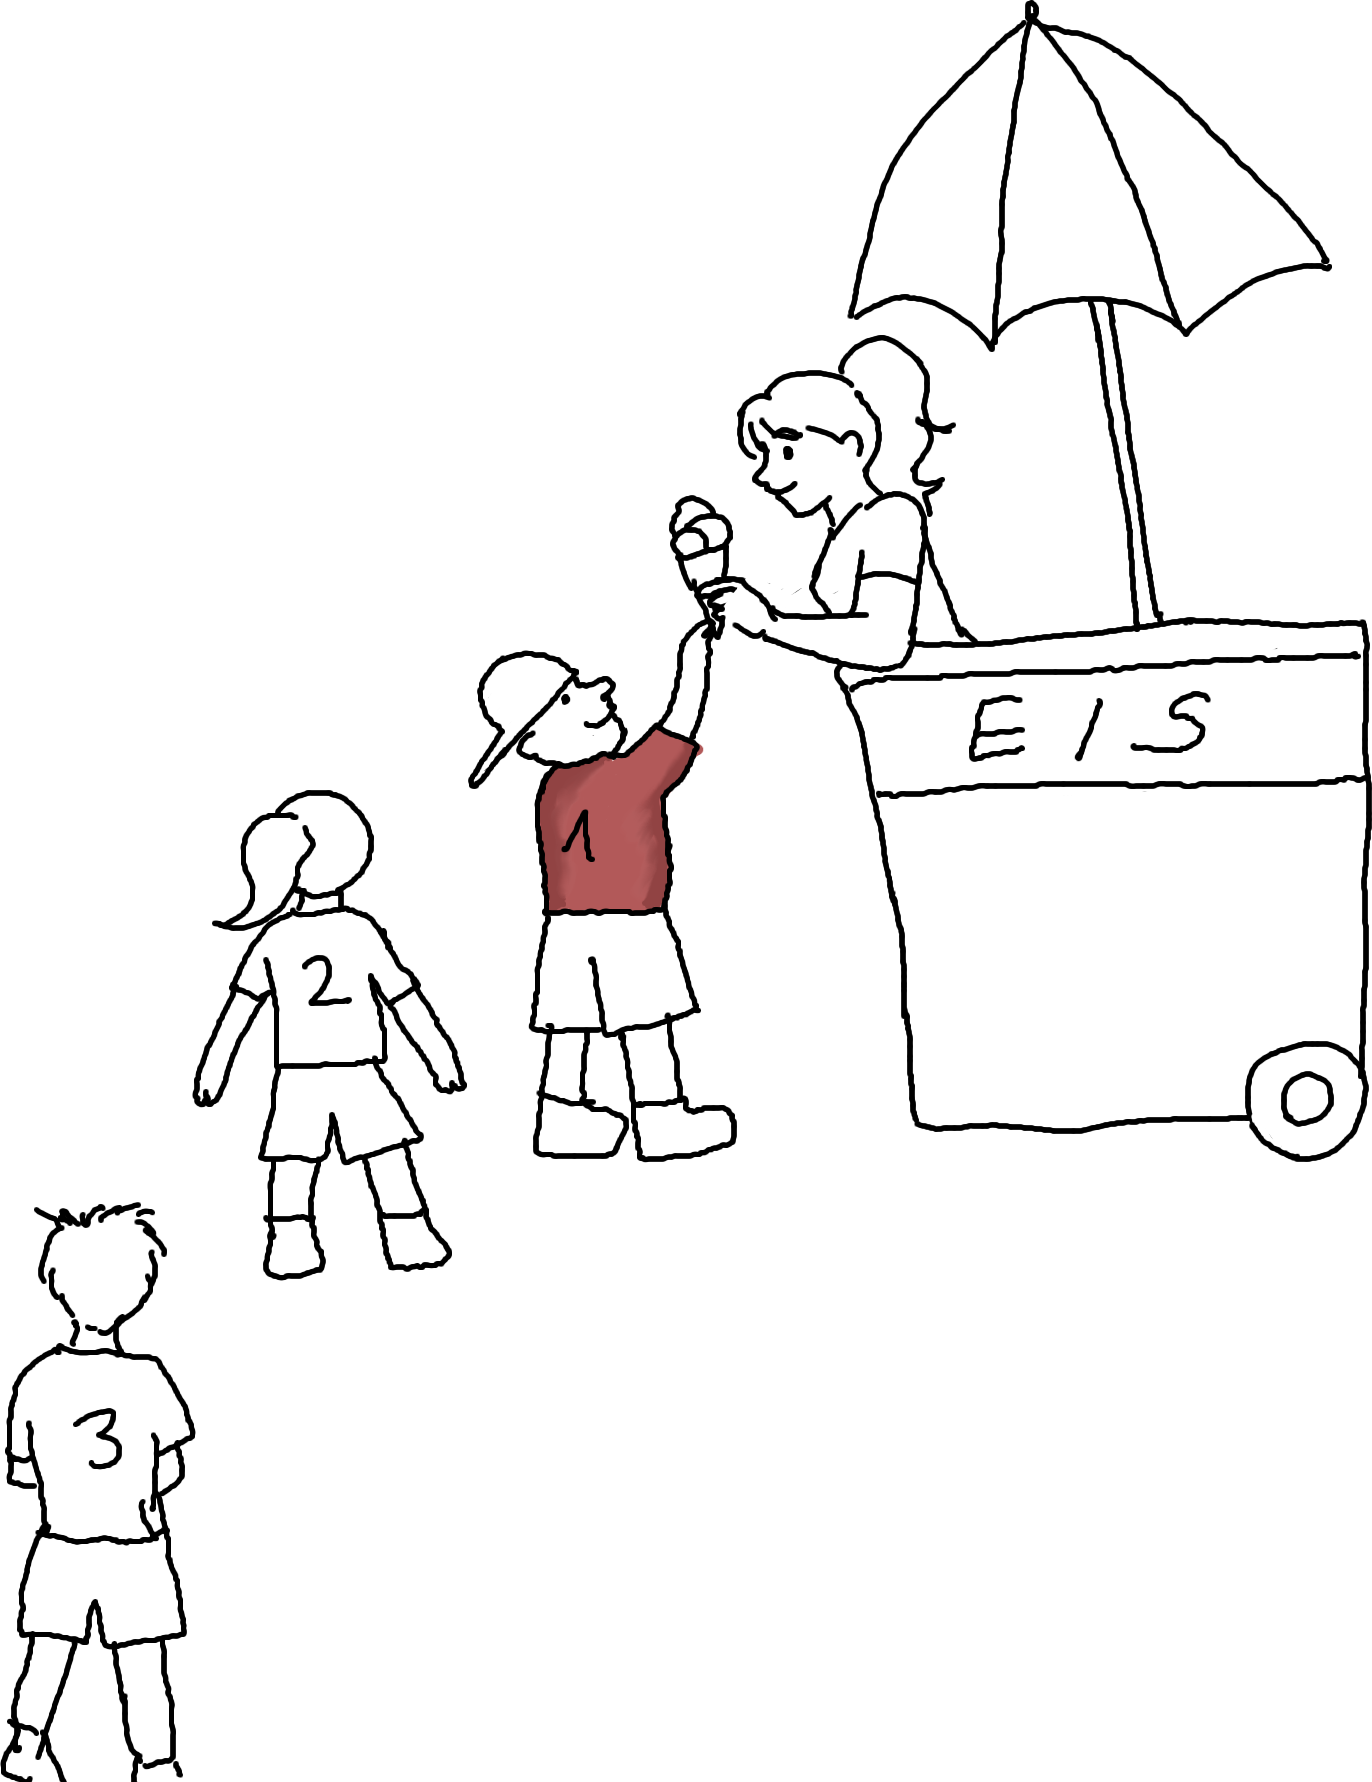
\includegraphics{infinite-queue}
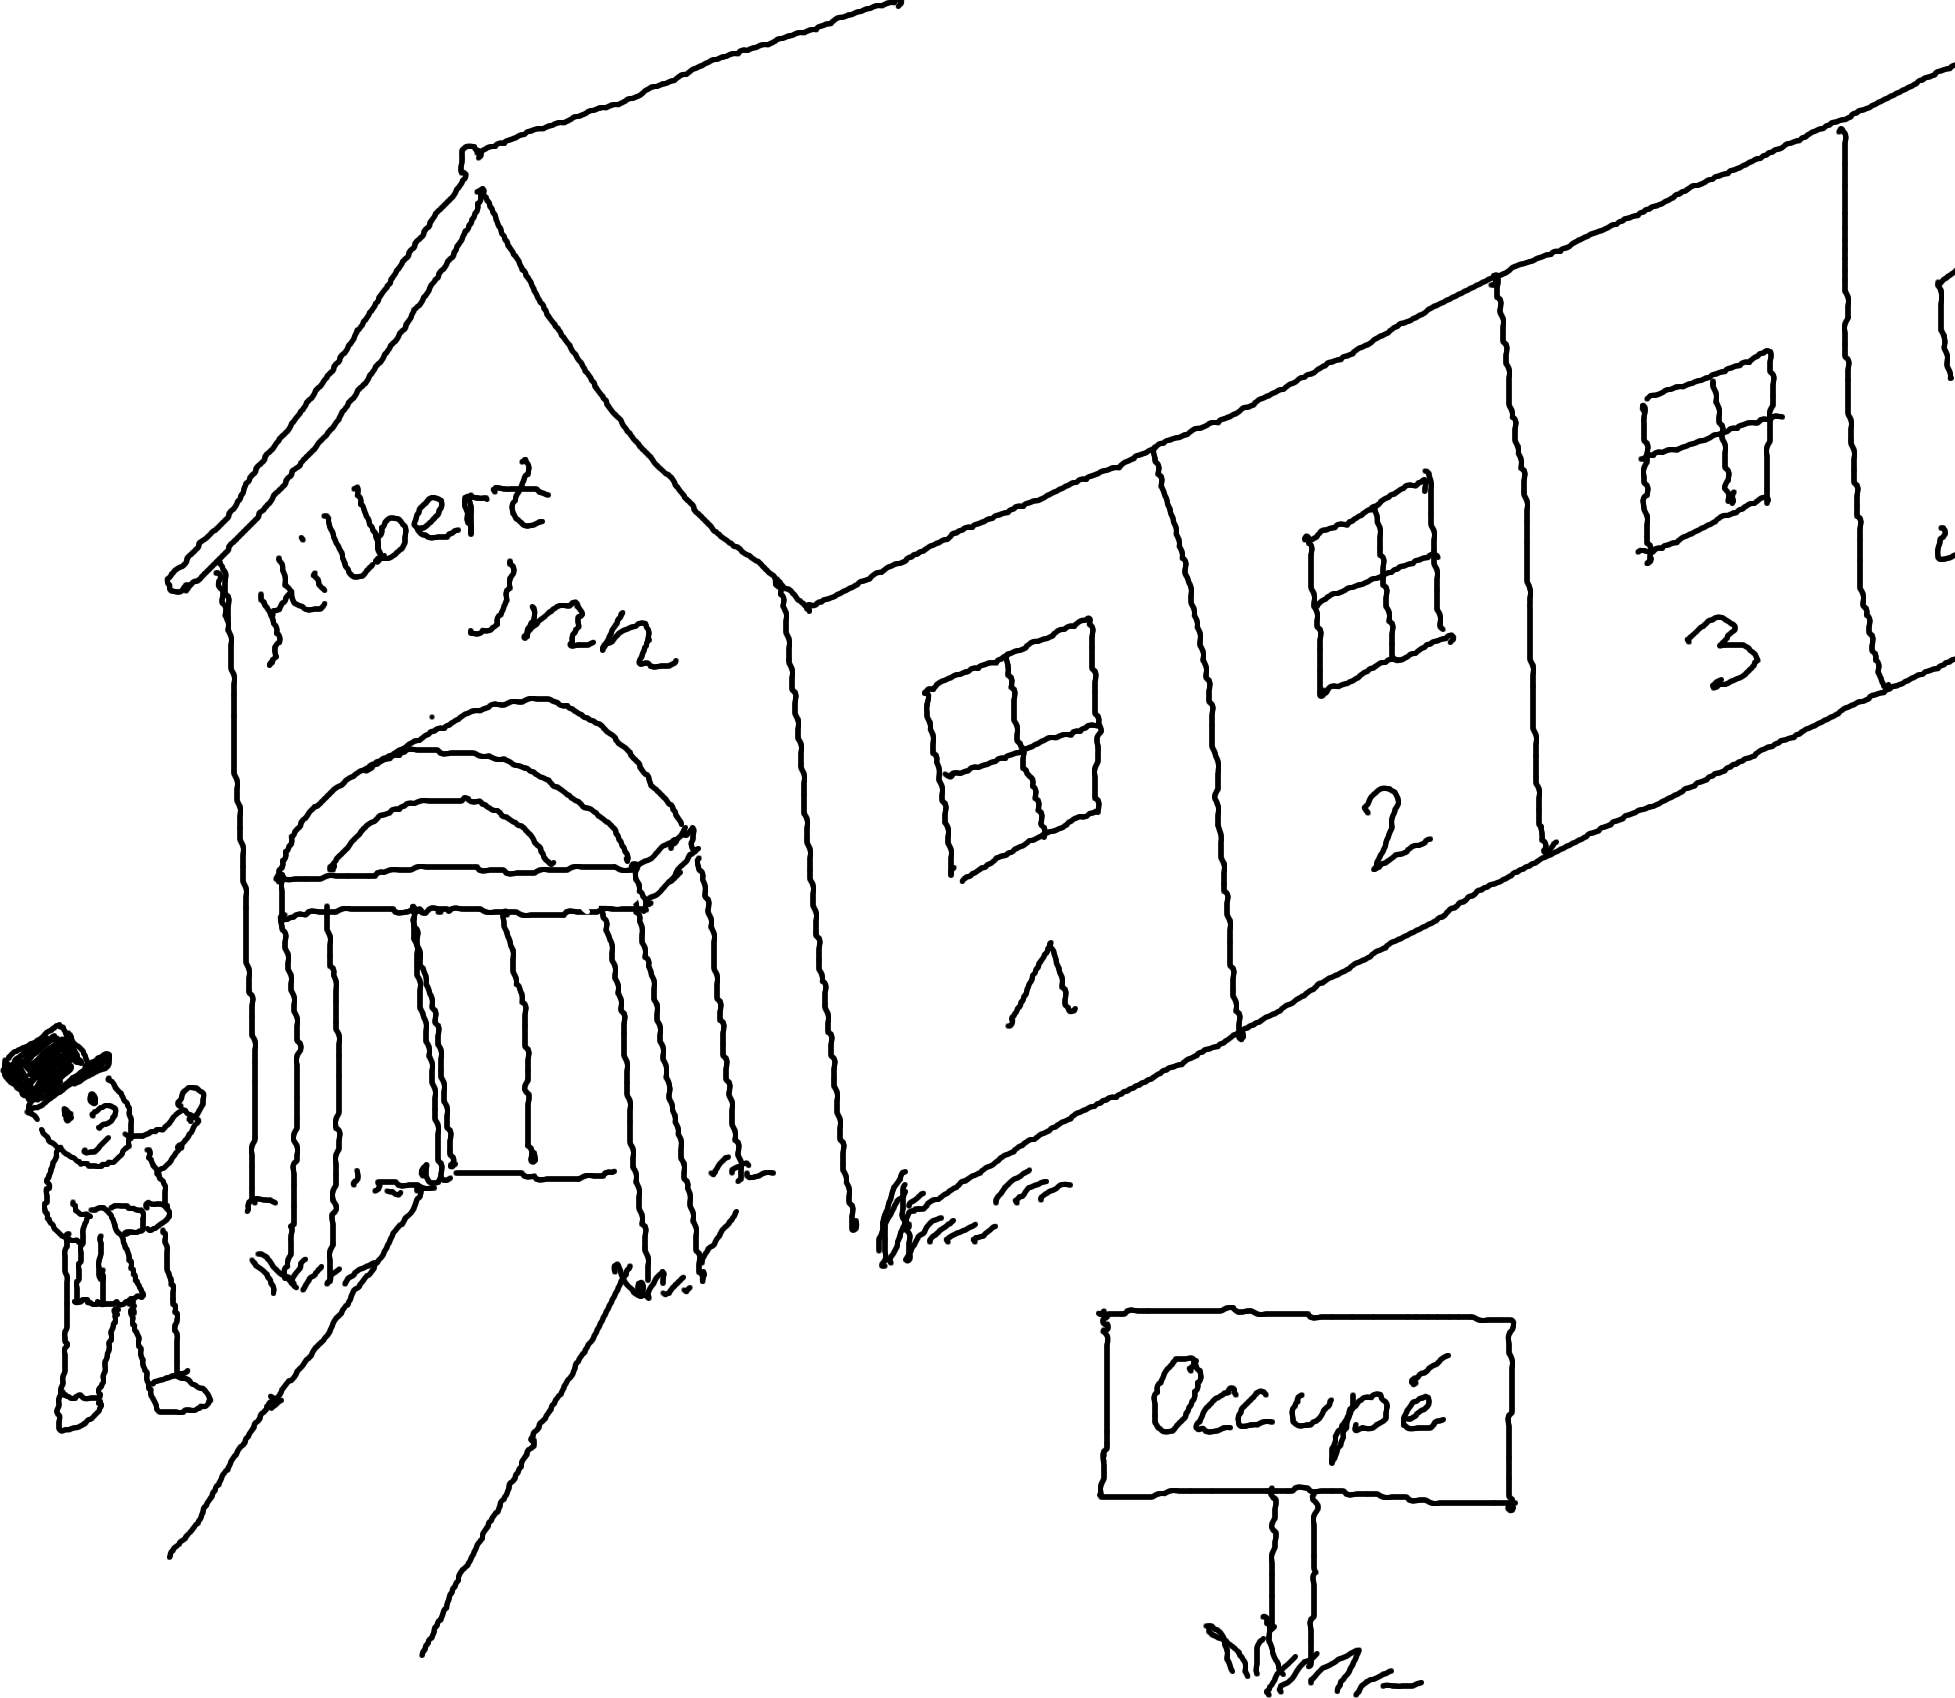
\includegraphics{hilberts-hotel}
